\chapter{Related Work}
In this section, we review recent approaches towards textual annotation. First we discuss available datasets, then multiple approaches in image classification. Lastly we examine object localization in an image. Unfortunately we did not include video annotation in out work since video processing and training creates unfeasible demands on computational power.

% and finally we look on image sequence annotation. Last part will be just a list of possible methods since all of them require unfeasible demands on computational power.

\section*{Datasets}
\addcontentsline{toc}{section}{Datasets}
Recent breakthroughs in machine learning could not happened without large-scale datasets since they are necessary to train and evaluate algorithms. Image datasets can be divided into three groups depending on what they are addressing:~image classification, object localization and semantic segmentation.

Objective of image classification tasks is to decide whether given object is or is not present on an image. There are multiple low-resolution datasets such as CIFAR-100~\cite{krizhevsky2009learning} containing 60,000 images in 100 categories with resolution 32-by-32 pixels. Since 2009 there is ImageNet~\cite{ILSVRC15}, a large-scale high resolution dataset with aims to populate the majority of the 80,000 WordNet synsets with 500 to 1000 images. In research a subset of the ImageNet database called ILSVRC2012 containing 1000 categories is usually used.

Task of object localization embodies stating what is in an image and where in the image it is. The location is usually given as an bounding box. As of 2018, ImageNet database holds bounding boxes for over 3000 synsets with an average of 150 images per synset. Similarly to ImageNet, Open Images Dataset~\cite{openimages} contains over one and half million annotated images with more than twice as many bounding boxes belonging into 600 categories. Semantic segmentation goes a step further. Its goal is to not only distinguish and localize object in an image but to assign each pixel to an object it is belonging to. Probably the most recognized dataset The Microsoft Common Objects in COntext (MS COCO)~\cite{lin2014microsoft} contains 91 common object categories with 82 of them having more than 5,000 labeled instances. There are also many more datasets focused on specific task such as Places~\cite{zhou2017places}, designed for scene recognition, or YFCC100M~\cite{YFCC100M} used for unsupervised learning.

\section*{Image Classification}
\addcontentsline{toc}{section}{Image Classification}
Prior to 2012 state-of-the-art approaches towards image classification involved using SVM classifiers trained on handcrafted features. Even though those methods can be tweaked, they rise and fall with a quality of the features. Since 2010 ImageNet Large Scale Visual Recognition Challenge (ILSVRC)~\cite{ILSVRC15} has been used to benchmark computer vision systems. Their dataset contains 1000 categories, each with around 1000 high resolution images. Top-5 error rate for the SVM classifiers hovered at over 25\% until in 2012 an entry from A.~Krizhevsky,~et~al.~\cite{AlexNet} disturbed machine learning community with by far the best result of 15.3\% using deep convolution neural network (DCNN) and pushed the whole industry towards neural networks, which until then were used only in limited number of cases such as handwritten character recognition. The main advantage of neural networks is that they, in contrast to a SVM classifiers, can learn the best features themselves and thus they seem ideal for such tasks. But we were unable to train larger models due to multiple issues that were overcome in the last few years.

Fast graphic cards, novel stochastic optimization algorithms \cite{kingma2014adam}, clever weight initialization \cite{glorot2010understanding}, non-saturating activation functions, dropout \cite{srivastava2014dropout} and many other techniques allowed for deeper and bigger networks.

\begin{figure}
	\centering

	\begin{tabular}{@{}c@{}}
		\subfloat{
			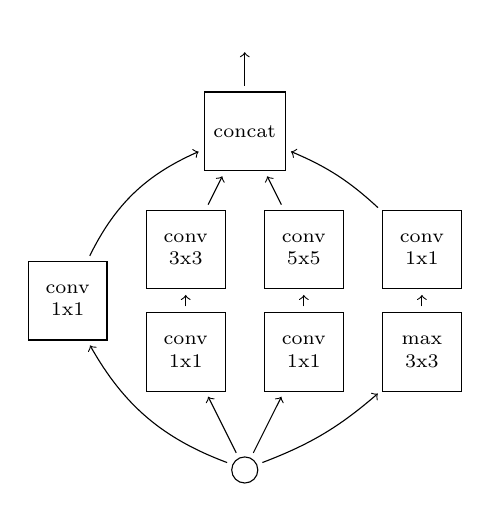
\begin{tikzpicture}[
box/.style={
	draw,
	minimum width=1cm,
	minimum height=1cm,
	font=\scriptsize,
	align=center
}, pil/.style={
	->,
	shorten <=2pt,
	shorten >=2pt
}]

\node[] (out) at (0,2.7) {};

\node[box] (concat) at (0,1.5) {concat};

\node[box] (bll) at (-2.25,-0.65) {conv \\ 1x1};

\node[box] (tl) at (-.75,0) {conv \\ 3x3};
\node[box] (tr) at (.75,0) {conv \\ 5x5};
\node[box] (trr) at (2.25,0) {conv \\ 1x1};

\node[box] (bl) at (-.75,-1.3) {conv \\ 1x1};
\node[box] (br) at (.75,-1.3) {conv \\ 1x1};
\node[box] (brr) at (2.25,-1.3) {max \\ 3x3};

\node[draw,circle] (input) at (0,-2.8) {};

\draw[pil] (concat) edge (out);

\draw[pil, bend left=20] (input) edge (bll);
\draw[pil] (input) edge (bl);
\draw[pil] (input) edge (br);
\draw[pil, bend right=10] (input) edge (brr);

\draw[pil] (bl) edge (tl);
\draw[pil] (br) edge (tr);
\draw[pil] (brr) edge (trr);

\draw[pil, bend left=20] (bll) edge (concat);
\draw[pil] (tl) edge (concat);
\draw[pil] (tr) edge (concat);
\draw[pil, bend right=10] (trr) edge (concat);
\end{tikzpicture}
		}
	\end{tabular}\qquad
	\begin{tabular}{@{}c@{}}
		\subfloat{
			\begin{tikzpicture}[scale=0.8,
box/.style={
	draw,
	minimum width=0.7cm,
	minimum height=0.7cm,
	font=\tiny,
	inner sep = 0pt,
	align=center
}, pil/.style={
	->,
	shorten <=2pt,
	shorten >=2pt
}, add/.style={
	draw,
	circle,
	inner sep = 0.2pt,
	font=\small,
	align=center
}]


\node[draw, diamond, font=\tiny, inner sep=0.5pt, align=center] (out) at (0,3.9) {$h_{i+1}$};

\node[box, inner sep=2pt] (concat) at (0,2.5) {concat};

\draw[pil] (concat) edge (out);

\node[add] (rr) at (4.2,1.1) {+};
\node[add] (r) at (2.1,1.1) {+};
\node[add] (c) at (0,1.1) {+};
\node[add] (l) at (-2.1,1.1) {+};
\node[add] (ll) at (-4.2,1.1) {+};

\draw[pil] (rr) edge (concat);
\draw[pil] (r) edge (concat);
\draw[pil] (c) edge (concat);
\draw[pil] (l) edge (concat);
\draw[pil] (ll) edge (concat);


\node[box] (rr1) at (4.68,0) {sep \\ 3x3};
\node[box] (rr2) at (3.72,0) {sep \\ 5x5};

\node[box] (r1) at (2.58,0) {avg \\ 3x3};
\node[box] (r2) at (1.62,0) {avg \\ 3x3};

\node[box] (c1) at (.48,0) {iden \\ tity};
\node[box] (c2) at (-.48,0) {avg \\ 3x3};

\node[box] (l1) at (-1.62,0) {sep \\ 5x5};
\node[box] (l2) at (-2.58,0) {sep \\ 3x3};

\node[box] (ll1) at (-3.72,0) {iden \\ tity};
\node[box] (ll2) at (-4.68,0) {sep \\ 3x3};

\draw[pil,out=90,in=315] (rr1) edge (rr);
\draw[pil,out=90,in=225] (rr2) edge (rr);

\draw[pil,out=90,in=315] (r1) edge (r);
\draw[pil,out=90,in=225] (r2) edge (r);

\draw[pil,out=90,in=315] (c1) edge (c);
\draw[pil,out=90,in=225] (c2) edge (c);

\draw[pil,out=90,in=315] (l1) edge (l);
\draw[pil,out=90,in=225] (l2) edge (l);

\draw[pil,out=90,in=315] (ll1) edge (ll);
\draw[pil,out=90,in=225] (ll2) edge (ll);


\node[draw, diamond, font=\tiny, inner sep=0.5pt, align=center] (h1) at (0,-1.4) {$h_{i-1}$};
\node[text height=0.333cm, execute at begin node=\color{black}$\vdots$] (hidden) at (0,-2.3) {};
\node[draw, diamond, font=\tiny, inner sep=0.5pt, align=center] (h2) at (0,-3.2) {$h_{i-2}$};

\draw[pil,out=135,in=270] (h1) edge (c2);
\draw[pil,out=180,in=270] (h1) edge (l1);
\draw[pil,out=180,in=270] (h1) edge (ll1);
\draw[pil,out=180,in=270] (h1) edge (ll2);


\draw[pil,out=30,in=270,dashed] (h2) edge (c1);
\draw[pil,out=180,in=270,dashed] (h2) edge (l2);
\draw[pil,out=0,in=270,dashed] (h2) edge (r1);
\draw[pil,out=0,in=270,dashed] (h2) edge (r2);
\draw[pil,out=0,in=270,dashed] (h2) edge (rr1);
\draw[pil,out=0,in=270,dashed] (h2) edge (rr2);
\end{tikzpicture}
		}
	\end{tabular}

	\caption[Various advanced DCNN architectures]{Inception block of GoogLeNet~\cite{szegedy2015going} (2014, left) and state-of-the-art block of NASNet-A~\cite{zoph2017learning} (2017, right). The later, created by a recurrent neural network, outperformed all blocks ever designed by people.}
	\label{fig:inception_block}
\end{figure}